\begin{doublespacing}

A finite element model is used to represent a area(2D) of an intragranular space. The 2D mesh is created using Trimesh. Two material objects are created, one being U-10Mo and another one is Xenon. Thermal conductivity of U-10Mo is used from Burkes et. al~\cite{burkes2010thermo}. Different set of thermal conductivity of Xenon is used. The effective thermal conductivity of 

\section{Introduction}
\begin{figure}[H]
\centering
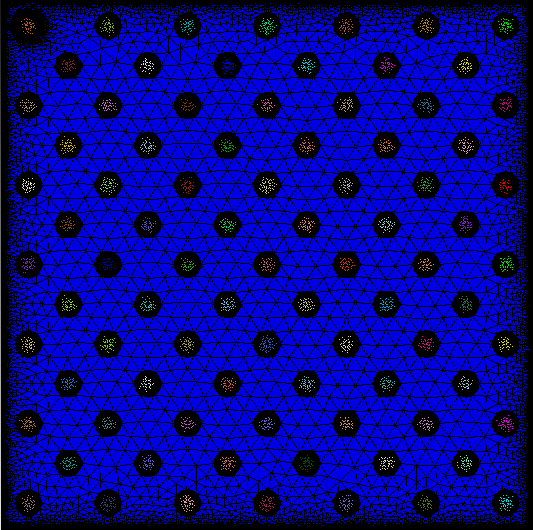
\includegraphics[scale=0.5]{fcc_mesh.png}
\caption{Meshed Xenon bubble inside U-10Mo matrix}
\label{fcc_mesh}
\end{figure}


\begin{figure}[H]
\centering
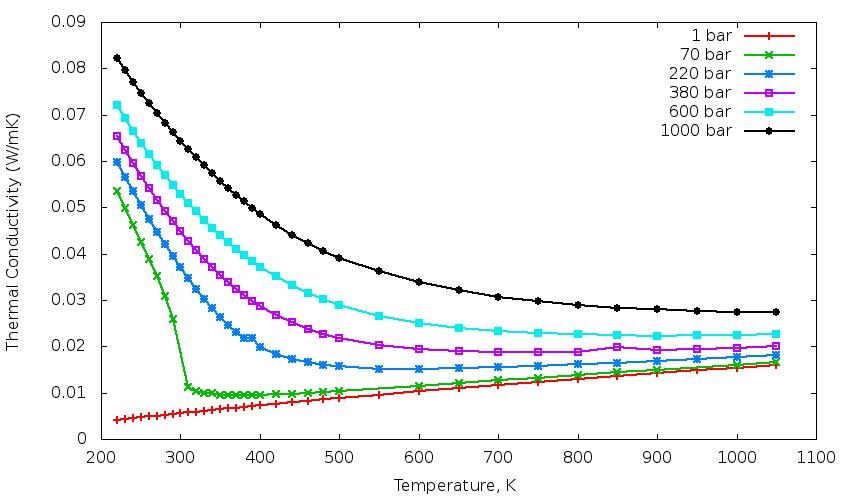
\includegraphics[scale=0.5]{Xe_K.png}
\caption{Thermal Conductivity of Xenon with increasing pressure}
\label{fig_Xe_K}
\end{figure}


\end{doublespacing}
